% Online Resource 1
\documentclass[pdflatex,sn-basic,Numbered]{sn-jnl}
\usepackage{graphicx,amsmath,amssymb,booktabs,array,tabularx}
\usepackage{xurl}
\usepackage[title]{appendix}
\usepackage{etoolbox}
\usepackage{flafter}
\usepackage[section]{placeins}
\urlstyle{same}
\setlength{\emergencystretch}{2em}
\raggedbottom
\AtBeginDocument{\hypersetup{
  pdftitle={Online Resource 1: Factorial Benchmarking of Exact and Finite-Shot Gradient Resolvability in a Four-Qubit Hybrid Quantum Neural Network},
  pdfauthor={Brandon Shen},
  pdfsubject={Supplementary Information for Discover Quantum Science}
}}

% Clean single-author correspondence formatting produced by sn-jnl.cls.
% Keep the conventional author asterisk while avoiding a duplicated asterisk
% on the affiliation, plural labels, and a trailing semicolon after the email.
\makeatletter
\patchcmd{\@maketitle}
  {Corresponding author(s). E-mail(s):}
  {Corresponding author:}
 {}{\PackageWarning{supplemental}{Could not patch corresponding-author label}}
\patchcmd{\email}
  {\textcolor{blue}{#1};\ }
  {\textcolor{blue}{#1}}
 {}{\PackageWarning{supplemental}{Could not remove corresponding-email semicolon}}
\makeatother
\begin{document}

\title{Online Resource 1: Factorial Benchmarking of Exact and Finite-Shot Gradient Resolvability in a Four-Qubit Hybrid Quantum Neural Network}
\author*[1]{\fnm{Brandon} \sur{Shen} (ORCID: \href{https://orcid.org/0009-0002-3545-2106}{0009-0002-3545-2106})}\email{brandonshen123@gmail.com}
\affil[1]{\orgname{Independent Researcher}, \orgaddress{\city{Belmont}, \state{California}, \country{United States}}}
\maketitle

\begin{center}
\textbf{Supplementary Information}
\end{center}

\section{Scope and frozen provenance}

This supplement accompanies the independently self-contained main manuscript. It preserves the corrected centered H1--H4 analyses, estimator diagnostics, numerical robustness checks, and the distinction between protocol-derived primary tests, previously frozen post-primary analyses, and explicitly later post-audit work. The machine-readable source of truth is \path{results/final_submission_v1/manifest.json}. The numerical-results freeze, \nolinkurl{submission-numerical-results-freeze-v1}, preserves the frozen scientific outputs. The accompanying OSF project is available at \href{https://doi.org/10.17605/OSF.IO/THV6G}{\nolinkurl{https://doi.org/10.17605/OSF.IO/THV6G}}. The distinct final manuscript/repository release, \href{https://github.com/Brandon-Shen/few-qubit-qnn-snr/tree/sndc-submission-v1}{\texttt{sndc-submission-v1}}, contains the preserved pre-remediation manuscript and supplement sources, code, documentation, verification scripts, and submission-facing repository state. Historical outputs under \path{results/superseded/}, \path{results/superseded_pooled/}, and other explicitly superseded directories are audit-only and are not current primary results. The post-audit sensitivity and correction records below are separate from that unchanged release.

\section{Scientific interpretation guide}

The primary experimental question is whether the specified CNOT schedule, terminal objective, and classical shortcut interact in initial gradient behavior within the implemented four-qubit measure--re-encode--reset architecture. The main manuscript presents the design and principal findings. This resource provides the full frozen numerical and inferential details, including results sensitive to the uncertainty procedure, estimator mode, depth weighting, or plug-in-SNR eligibility. The interpretation of the corrected primary family is: H1, positive $E\times L$ interaction in $\operatorname{asinh}(|g^{\mathrm{exact}}|)$ supported by Wald/Holm and initialization-cluster bootstrap inference, directionally corroborated under an independent seed set; H2, finite-shot $E\times L$ interaction supported by the Wald/Holm rule but not by its nested-bootstrap interval; H3, finite-shot $E\times R$ interaction with the same inferential disagreement and additional estimator-mode sensitivity; H4, unresolved $L\times R$-by-hybrid-block-count moderation. A non-rejection is not evidence of an exactly zero effect. A separately labeled post-audit vector-preserving sensitivity with 1,000 accepted fits also leaves H2--H4 and simple H3 intervals spanning zero; it is not a preregistered replacement analysis.

The coefficient descriptions concern defined regression response scales and the specified model terms; they are not universal physical effects. In particular, block count $D$ is not uninterrupted coherent circuit depth, the $L$ contrast changes the entire objective and measurement construction, and matched simulator-shot totals are not matched physical-resource costs. Classical parameter gradients and training trajectories are outside H1--H4. These scope conditions also govern interpretation of the diagnostic and post-primary results below.

\section{Factor-coding correction and estimands}

The adopted factors are
\[
E_c=E-\tfrac12,\qquad L_c=L-\tfrac12,\qquad R_c=R-\tfrac12,
\]
with values $\{-1/2,+1/2\}$. Hybrid block count is standardized as $D_z=(D-3.2)/1.7204650534085253$, where 3.2 and 1.7204650534085253 are respectively the mean and population standard deviation of $D\in\{1,2,3,4,6\}$. Because $E_cL_cR_c$ remains in each applicable model, centered lower-order interactions average equally over the third binary factor. Direct-0/1 lower-order coefficients instead describe simple interactions at the third factor's reference level. The parameterizations yield identical fitted values, likelihood, residuals, and random effects; only the interpretation of lower-order coefficients changes. The correction was an implementation--interpretation correction rather than result-dependent model selection. H1 and H2 use $E_cL_c$, H3 uses $E_cR_c$ averaged over $L$, and H4 uses $L_cR_cD_z$.

\section{Implemented forward pass, dimensions, and SNR definition}

For each nonterminal block $\ell<D$, $x^{(\ell)},z^{(\ell)},\theta^{(\ell)}\in\mathbb{R}^4$, $W_\ell\in\mathbb{R}^{4\times4}$, and $b_\ell\in\mathbb{R}^4$. The code sets $x^{(1)}=z^{(0)}=0$. Each block resets to $|0000\rangle$, applies $R_y(\theta_q^{(\ell)}+x_q^{(\ell)})$ for $q=0,\ldots,3$, and then applies its four ordered CNOTs. For $\ell<D$, a common Z-basis measurement returns all four $z_j^{(\ell)}=\langle Z_j\rangle$ and $x^{(\ell+1)}=W_\ell z^{(\ell)}+b_\ell+\gamma z^{(\ell-1)}$, with $\gamma=R$. The terminal block is evaluated directly with the selected objective (global ground-state infidelity for $L=0$ or normalized TFIM energy for $L=1$), not converted into another inter-block feature vector. There is no clipping, wrapping, normalization, nonlinearity, or rescaling. The $4D$ quantum-rotation derivatives enter H1--H4; the $20(D-1)$ classical $W,b$ derivatives do not.

Quantum angles are independent $\mathrm{Uniform}(0,2\pi)$ draws. Each $W_\ell$ is Glorot-uniform on $[-\sqrt{6/8},\sqrt{6/8}]$ and every $b_\ell$ is zero. Quantum, classical, shot, and bootstrap namespaces are separately derived with SHA-256, but the finite shot-seed space has the cross-cell reuse documented below. All configurations at fixed initialization and $D$ reuse identical arrays and indices; distinct $D$ values use depth-specific seeds and do not share shallow prefixes.

The 31-bit reduction of derived shot seeds produced 70 two-use seed groups (70 excess assignments, involving 140 vectors) among 480,000 requests, with 479,930 distinct seeds. No repeated seed occurred within a scientific cell. Of the 19 end-to-end/end-to-end pairs, 18 cross initialization clusters; 14 pairs are conditional/conditional and 37 are cross-mode. No compared pair had identical complete archived gradient vectors; individual shot outcomes are unavailable. The induced inferential effect remains unmeasured. The whole-vector sensitivity preserves these frozen streams and does not establish complete initialization-cluster independence. Matching of quantum/classical initial parameters and exact H1 are separate from this shot-stream defect. These counts and mappings are retained in \path{verification/independent_audit/remediation/stage2_20261112_rng_pilot/rng_summary.json}.

\begin{figure*}[t]\centering
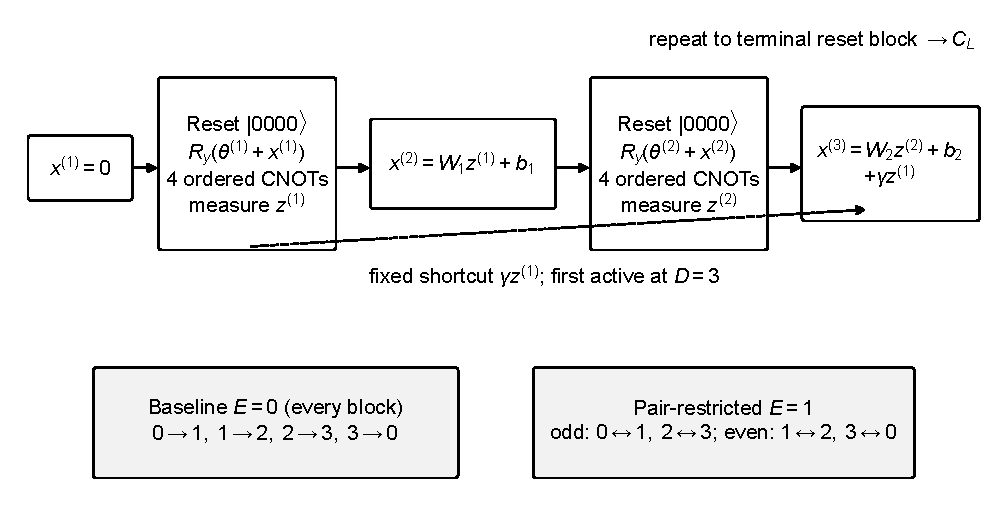
\includegraphics[width=.94\textwidth]{fig16_architecture.pdf}
\caption{Code-verified reset-per-block forward pass. Solid arrows transmit four-dimensional classical features; the dashed fixed-gain shortcut is active only for $R=1$ and first changes the third block input. Every quantum box starts with a reset register. Baseline and pair-restricted CNOT schedules are shown without implying continuous quantum-circuit depth across blocks}
\label{supp:fig:architecture}
\end{figure*}

At fixed parameters, the population target of the complete finite-shot gradient estimator is $\mathrm{SNR}^{*}_{\mathrm{est},k}=|\mu_k|/\sigma_k$, where $\mu_k$ and $\sigma_k^2$ are the repeated-shot mean and variance of the complete gradient estimator. The analyzed plug-in quantity is
\[
\widehat{\mathrm{SNR}}_{\mathrm{est},k}=|\bar g_k|/s_k,
\quad s_k^2=\frac{1}{29}\sum_{r=1}^{30}(\hat g_{kr}-\bar g_k)^2.
\]
Duplicate replicate keys and invalid rows are rejected before aggregation; the frozen validation reported neither. When $s_k=0$, the mathematical plug-in ratio $|\bar g_k|/s_k$ is undefined if $\bar g_k=0$ and unbounded in the extended-real sense if $\bar g_k\ne0$. The implementation records NaN and positive infinity, respectively; both cases are ineligible for the primary finite-SNR regression analysis, without an epsilon or variance floor. The labeled include-zero sensitivity assigns zero only when both $\bar g_k=0$ and $s_k=0$. H2--H4 concern this finite-replicate plug-in ratio, not the mean-estimate $t$-statistic $\sqrt{30}\,\bar g_k/s_k$. Estimator bias is $\mu_k-g_k^{\mathrm{exact}}$, whose plug-in estimate is $\bar g_k-g_k^{\mathrm{exact}}$; empirical sign agreement uses $\bar g_k=30^{-1}\sum_{r=1}^{30}\hat g_{kr}$ and is false if either $\bar g_k$ or $g_k^{\mathrm{exact}}$ is zero, including when both are zero. It is distinct from the population mean-sign comparison and from a fraction of replicate signs. Neither SNR nor sign agreement by itself establishes optimization success.
\[
\mathbb{1}\!\left[\begin{gathered}
\bar g_k\ne0,\quad g_k^{\mathrm{exact}}\ne0,\\
\operatorname{sign}(\bar g_k)=\operatorname{sign}(g_k^{\mathrm{exact}})
\end{gathered}\right].
\]

\section{Corrected primary family and bootstrap}

\begin{table*}[t]
\centering
\footnotesize
\begin{tabularx}{\textwidth}{@{}l p{0.13\textwidth} r l r l >{\raggedright\arraybackslash}X@{}}
\toprule
Hyp. & Estimand & Estimate & Wald 95\% CI & Holm $p$ & Bootstrap 95\% CI & Evidence \\
\midrule
H1 & $E_cL_c$, exact
   & 0.004043
   & \mbox{$[0.001924,\,0.006162]$}
   & 0.000739
   & \mbox{$[0.000473,\,0.007535]$}
   & Both \\
H2 & $E_cL_c$, end-to-end
   & 0.014338
   & \mbox{$[0.004255,\,0.024422]$}
   & 0.015963
   & \mbox{$[-0.016240,\,0.045992]$}
   & Wald only \\
H3 & $E_cR_c$, end-to-end
   & -0.011615
   & \mbox{$[-0.021697,\,-0.001534]$}
   & 0.047875
   & \mbox{$[-0.031375,\,0.009563]$}
   & Wald only \\
H4 & $L_cR_cD_z$
   & -0.010179
   & \mbox{$[-0.020688,\,0.000331]$}
   & 0.057658
   & \mbox{$[-0.025964,\,0.005863]$}
   & Neither \\
\bottomrule
\end{tabularx}
\caption{Original frozen corrected primary family. Wald intervals and Holm-adjusted $p$-values follow the primary model-based decision rule. Bootstrap intervals use initialization-cluster resampling for H1 and nested initialization-cluster/within-cell replicate resampling for H2--H4. ``Both'' means that the Wald and bootstrap intervals exclude zero; ``Wald only'' means that the Wald/Holm rule rejects while the bootstrap interval includes zero; and ``Neither'' means that the Wald/Holm rule does not reject and the bootstrap interval includes zero. H1 used 2,000 completed fits with zero failures; H2--H4 used exactly 1,000 unique valid fits. The original finite-shot column retains component-wise inner resampling; post-audit vector-preserving intervals are in Section~\ref{supp:sec:vector-bootstrap}. Bootstrap iterations are distinct from the 50 top-level initialization clusters.}
\label{supp:tab:primary}
\end{table*}

For the original adopted H2--H4 bootstrap, outer resampling selected complete initialization clusters and retained all configurations, depths, budgets, and matched parameters; within selected parameter-level scientific cells, finite-shot replicates were independently resampled and SNR was recomputed before refitting. H1 resampled complete initialization clusters. Percentile intervals are reported without treating either Wald or bootstrap inference as universally preferable. Shared within-vector measurement noise was consequently not preserved across parameter components in that original inner procedure.

The frozen finite-shot production dataset used 30 finite-shot vector replicates per initialization/configuration/depth/budget/mode cell and 50 independently initialized top-level design clusters, with the cross-cell shot-stream reuse qualified above. The separately seeded replicate-count diagnostic began at 30 on representative cells. It tested signed-mean and SNR width tolerances, but explicitly checked stability only for signed-mean width; a nonfinite SNR half-width is treated as passing that code branch and does not establish precision. Four depth-one cells remained unresolved through the $R_{\mathrm{rep}}=200$ search ceiling; the overall return of 200 includes fallback and is not a successful uniform calibration. Production retained 30, with no recollection. The recorded diagnostics inform precision limitations rather than establish prospectively calibrated production counts.

The archived initialization-count calculation used fitted assumptions matching the production end-to-end model; a committed repository account records regeneration after the estimator-mode correction. No distinct independent, excluded initialization-pilot input or original decision chronology is established. Only $N_{\mathrm{init}}=50$ is recorded; 25 was the configured increment, not evidence that larger candidates were evaluated. The recorded 90th-percentile simulated Wald 95\% CI half-widths were 0.1026212747780318 for $E{:}L$, 0.10253728880520716 for $E{:}R$, and 0.07250672321768473 for $L{:}R{:}\mathrm{depth}_z$, each below 0.20. This operational transformed-scale precision threshold is not an equivalence margin or scientific-importance claim. The calculation used historical direct-coded finite-shot interactions and did not evaluate H1 or prospectively size the later centered primary family. Its current archived form is a retrospective precision diagnostic, not proof of independent pilot-based selection.

The original adopted H2--H4 pool preserves the earlier 443 successful draws unchanged (8 validated draws plus three independently seeded 145-draw shards) and appends non-overlapping deterministic continuation draws to reach exactly 1,000 unique valid fits under the revised stopping instruction. A further 178 valid fits completed before workers stopped; they are preserved in the superseded audit location and excluded from all original adopted intervals. The 443-fit result remains an audit checkpoint, not the final result. Machine-readable provenance files record attempted, included-successful, excluded-successful, failed, and rejected counts, global iteration IDs, shard seeds, convergence status, and coefficient vectors. These counts refer to completed bootstrap fits, not independent initialization clusters. Original percentile endpoints retain finite Monte Carlo uncertainty; the distinct post-audit sample below contains none of these original or diagnostic-pilot draws.

\begin{table*}[t]\centering\small
\begin{tabular}{crrr}
\toprule
Completed fits & H2 $E_cL_c$ interval & H3 $E_cR_c$ interval & H4 $L_cR_cD_z$ interval \\
\midrule
40    & [-0.011931, 0.035640] & [-0.028213, 0.000850] & [-0.024829, 0.006450] \\
100   & [-0.019772, 0.041956] & [-0.033480, 0.009079] & [-0.027224, 0.005826] \\
200   & [-0.017723, 0.044496] & [-0.032630, 0.006696] & [-0.024829, 0.005711] \\
400   & [-0.016692, 0.043008] & [-0.030956, 0.010311] & [-0.026885, 0.006433] \\
443   & [-0.016638, 0.043563] & [-0.030943, 0.010259] & [-0.026975, 0.006403] \\
1,000 & [-0.016240, 0.045992] & [-0.031375, 0.009563] & [-0.025964, 0.005863] \\
\bottomrule
\end{tabular}
\caption{H2--H4 nested-bootstrap percentile endpoint checkpoints. Every interval includes zero. The 443 row is the preserved historical checkpoint; 1,000 is the final included fit count. Rows are cumulative completed refits of resampled data, not independent datasets; endpoint movement reflects finite Monte Carlo uncertainty. Order-statistic/binomial-rank endpoint diagnostics in the machine-readable summary quantify Monte Carlo uncertainty and are not scientific confidence intervals.}
\label{supp:tab:bootstrap-checkpoints}
\end{table*}

\section{Post-audit vector-preserving bootstrap sensitivity}\label{supp:sec:vector-bootstrap}
The independent audit confirmed that the original inner resampling discarded cross-parameter dependence from shared vector measurements and reverse assembly. The separately authorized post-audit routine resampled complete 30-by-$(4D)$ matrices by replicate row, preserving the same selected row and multiplicity across all parameters within each initialization copy, configuration, depth, budget and mode. The outer draw remained 50 complete matched initialization clusters with uniquely relabeled copies. Different configurations, depths, budgets and modes retained separate inner streams. SNR, exact-zero/nonfinite eligibility, centered-equivalent model, REML, and random-effects structure were unchanged.

The full sensitivity used deterministic master seed 2026112103, separate from pilot seed 2026111203, and included 1,000 accepted fits from 1,000 attempts with no failures, rejections or interruptions. Diagnostic-pilot and original bootstrap draws were excluded. All accepted fits converged; 26 used optimizer fallback and one converged draw met the existing $10^{-8}$ singularity flag. That draw was retained under the unchanged acceptance policy, not removed to improve an interval. This is post-audit evidence, not a preregistered or protocol-derived primary family. H1 was not refit.

\begin{table*}[t]\centering\small
\begin{tabular}{lcc}
\toprule
Quantity & Original adopted 95\% interval & Post-audit vector 95\% interval \\
\midrule
H2 & $[-0.016240,0.045992]$ & $[-0.015673,0.045908]$ \\
H3 & $[-0.031375,0.009563]$ & $[-0.032595,0.008511]$ \\
H4 & $[-0.025964,0.005863]$ & $[-0.026397,0.007255]$ \\
H3, $L=0$ & $[-0.029117,0.024560]$ & $[-0.030918,0.025868]$ \\
H3, $L=1$ & $[-0.049490,0.007197]$ & $[-0.048136,0.009100]$ \\
H3, objective-average & $[-0.031375,0.009563]$ & $[-0.032595,0.008511]$ \\
\bottomrule
\end{tabular}
\caption{Original adopted component-wise and post-audit vector-preserving percentile 95\% intervals, each from 1,000 accepted fits. Every interval includes zero. The objective-average H3 row duplicates H3 and is not an additional test. Simple H3 contrasts are post-primary. The original primary table and Holm family are unchanged.}
\label{supp:tab:vector-bootstrap}
\end{table*}

No H2--H4 or simple H3 zero-crossing classification changed, although endpoints, widths and coefficient distributions differed. This comparison does not establish nominal coverage or isolate the effect of the frozen cross-cluster RNG reuse. Historical and new draws use different deterministic streams and their distribution comparison is unpaired; finite Monte Carlo variation contributes to observed differences. Binomial/order-statistic endpoint Monte Carlo ranges quantify simulation precision of each percentile endpoint, not additional scientific confidence intervals. No method or stopping rule was selected for significance.

The finalized report, \path{procedure_comparison.csv}, \path{sensitivity_coefficients.csv}, \path{fit_status.csv}, and \path{endpoint_monte_carlo_rank_intervals.csv} are under \path{verification/independent_audit/remediation/stage3_20261121_full_vector_sensitivity/analyses/finalization_0000/}. The four filenames in this paragraph are relative to that directory. Source/code/plan hashes and complete per-attempt lineage are retained in the parent run directory. Original adopted estimates, Wald/Holm results, bootstrap intervals and frozen metadata remain unchanged.

\section{Independent-seed H1 and depth weighting}

The independent-seed centered H1 estimate was $0.007726$ (Wald 95\% CI $[0.005592,0.009860]$); its 2,000-fit, zero-failure bootstrap interval was $[0.003402,0.011923]$. The direction was retained but magnitude remained uncertain.

\begin{table*}[t]
\centering\small
\resizebox{\textwidth}{!}{%
\begin{tabular}{crrrr}
\toprule
$D$ & Original estimate & Original 95\% CI & Independent-seed estimate & Independent-seed 95\% CI \\
\midrule
1 & -0.005251 & [-0.013708, 0.003206] & 0.001862 & [-0.006653, 0.010378] \\
2 & -0.003579 & [-0.009560, 0.002401] & 0.003120 & [-0.002901, 0.009141] \\
3 & 0.012588 & [0.007706, 0.017471] & 0.006250 & [0.001334, 0.011166] \\
4 & 0.004664 & [0.000435, 0.008892] & 0.007885 & [0.003627, 0.012143] \\
6 & 0.003446 & [-0.000007, 0.006898] & 0.010870 & [0.007393, 0.014346] \\
\midrule
Equal depth & 0.002374 & [-0.000164, 0.004911] & 0.005997 & [0.003443, 0.008552] \\
Observation/parameter weighted & 0.004043 & [0.001929, 0.006157] & 0.007726 & [0.005597, 0.009854] \\
\bottomrule
\end{tabular}}
\caption{Post-primary H1 depth contrasts and weighting summaries. Observation and matched-parameter weights are identical: 0.0625, 0.125, 0.1875, 0.25, and 0.375 at $D=1,2,3,4,6$. Intervals are unadjusted Wald 95\% intervals.}
\label{supp:tab:h1-depth}
\end{table*}

In the original dataset, moderation tests were mixed-model $\chi^2(4)=22.844$, $p=0.000136$, and cluster-robust $\chi^2(4)=6.008$, $p=0.1985$. Independent-seed tests were $\chi^2(4)=7.563$, $p=0.1090$, and $\chi^2(4)=1.810$, $p=0.7706$. The original-dataset depth conclusion is covariance-sensitive; cross-seed magnitude differences have no clear depth localization under the frozen rule.

\begin{figure*}[t]\centering
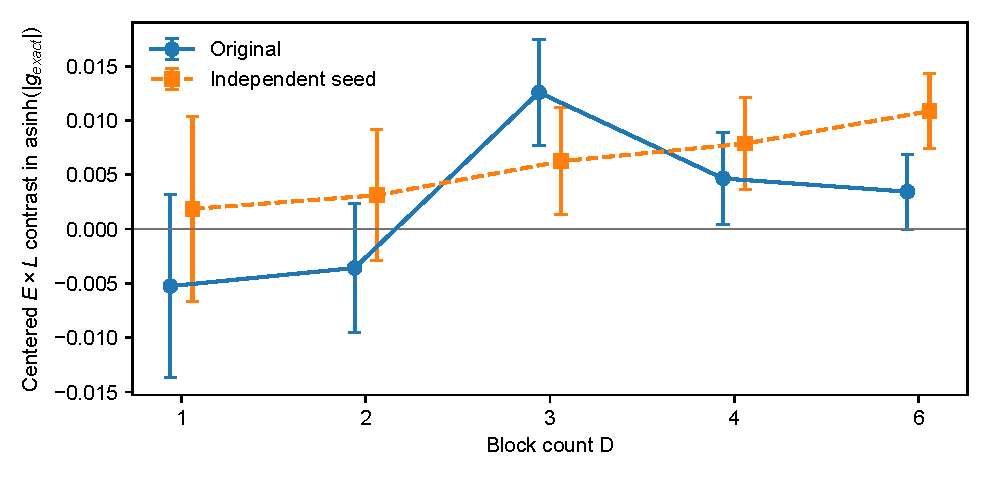
\includegraphics[width=.75\textwidth]{fig13_h1_depth.pdf}
\caption{Post-primary centered H1 contrasts by block count. Bars are unadjusted Wald 95\% intervals; zero is the reference. Dataset identity is encoded by shape and line style, not color alone. No monotonic depth law is assumed}
\end{figure*}

\begin{figure*}[t]\centering
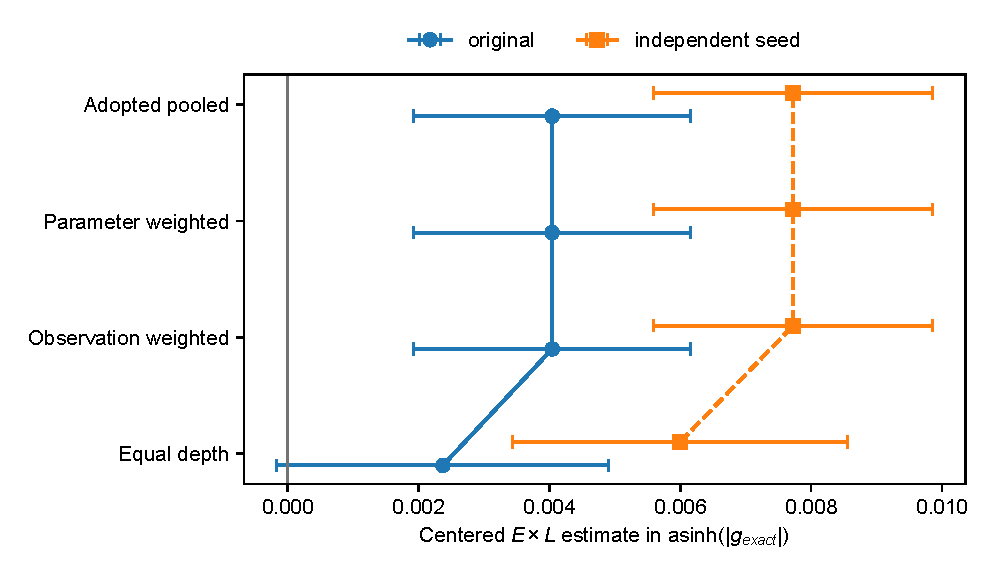
\includegraphics[width=.75\textwidth]{fig14_h1_weighting.pdf}
\caption{Post-primary equal-depth, observation/matched-parameter, and adopted pooled H1 summaries. Bars are Wald 95\% intervals. Weightings answer different questions and were not selected by significance}
\end{figure*}

\section{H3 post-primary explanatory analyses}

\begin{table*}[t]
\centering\small
\begin{tabular}{lrrr}
\toprule
Contrast or sensitivity & Estimate & Wald 95\% CI & Bootstrap 95\% CI \\
\midrule
End-to-end, $L=0$ & -0.000958 & [-0.015251, 0.013336] & [-0.029117, 0.024560] \\
End-to-end, $L=1$ & -0.022273 & [-0.036493, -0.008052] & [-0.049490, 0.007197] \\
End-to-end, L-average & -0.011615 & [-0.021697, -0.001534] & [-0.031375, 0.009563] \\
Active depths $D\ge3$, L-average & -0.014788 & [-0.024480, -0.005095] & Not planned \\
Conditional mode, L-average & 0.006978 & [-0.004745, 0.018701] & Not available \\
\bottomrule
\end{tabular}
\caption{Post-primary H3 explanatory and sensitivity results. The original adopted 1,000-fit bootstrap intervals contain zero for both objective-specific contrasts and their average. Active-depth and conditional-mode rows are not substitutions for the primary model. Post-audit intervals are separately reported in Section~\ref{supp:sec:vector-bootstrap}.}
\end{table*}

Depth-specific L-averaged estimates at $D=1,2,3,4,6$ were $0.006642$, $0.000696$, $-0.026492$, $-0.011553$, and $-0.011255$. Joint moderation did not reject with model-based ($p=0.545$) or cluster-robust ($p=0.721$) covariance. All 50 leave-one-initialization-out fits completed; all retained the negative averaged sign, 41 had raw $p<0.05$, and estimates ranged from $-0.014433$ to $-0.008562$. These diagnostics do not justify deletion. The frozen classification is a model-dependent directional signal, objective-specific under end-to-end mode.

\section{Conditional exact-gradient indices}

The frozen descriptive indices are
\[
J_{EL\mid R=0}=\frac{G_{EL}G_0}{G_EG_L},\qquad
J_{EL\mid R=1}=\frac{G_{ELR}G_R}{G_{ER}G_{LR}}.
\]
Unique exact-gradient parameter rows are pooled before the configuration-level RMS construction, so deeper depths receive more observation/parameter weight. The indices are conditional on $R$, not transformations of centered coefficients.

\begin{table}[t]\centering\small
\begin{tabular}{llrrr}
\toprule
Dataset & Estimand & Point & Median & Percentile 95\% CI \\
\midrule
Original & $J_{EL\mid R=0}$ & 1.241760 & 1.238674 & [1.082210, 1.414864] \\
Original & $J_{EL\mid R=1}$ & 1.126633 & 1.124329 & [0.991331, 1.285152] \\
Independent seed & $J_{EL\mid R=0}$ & 1.163219 & 1.160949 & [1.007100, 1.352596] \\
Independent seed & $J_{EL\mid R=1}$ & 1.242137 & 1.238157 & [1.049874, 1.449258] \\
\bottomrule
\end{tabular}
\caption{Conditional descriptive exact-gradient indices. Each initialization-cluster bootstrap completed 2,000 iterations with zero failures. Values above one are above the multiplicative no-interaction reference, not percentage improvements in optimization.}
\end{table}

\begin{figure}[t]\centering
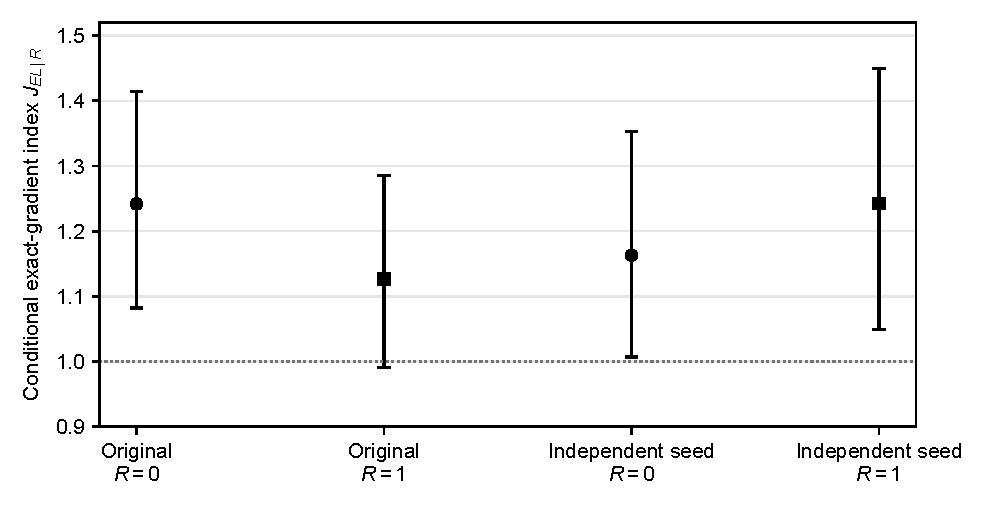
\includegraphics[width=.75\textwidth]{fig12_j_conditional.pdf}
\caption{All four frozen conditional $J_{EL\mid R}$ estimates with percentile 95\% bootstrap intervals and reference line $J=1$. Marker shape identifies $R$ and axis labels identify the dataset; the interval stems are solid. These are descriptive secondary ratios}
\end{figure}

\section{Prepared-state metrics at initialization}

After deduplication across shot budgets, the frozen table contains 4,000 terminal-block prepared-state records with unique dataset/initialization/configuration/depth keys. Physical quantum-state uniqueness was not independently established. Fidelity and normalized-energy bounds, row uniqueness, energy spectral bounds, and fidelity--infidelity complementarity all passed. Original configuration--depth mean fidelity ranged approximately 0.0338--0.0817 and normalized energy 0.4631--0.5529; independent-seed ranges were 0.0322--0.0962 and 0.4561--0.5537. The ranges overlap strongly. Since $L$ changes evaluation rather than preparation, paired $L=0$/$L=1$ prepared-state summaries are identical. No significance test or causal gradient--task relationship is inferred.

\begin{table}[t]
\centering
\small
\begin{tabular}{lcc}
\toprule
Dataset & Cell-mean fidelity range & Cell-mean normalized-energy range \\
\midrule
Original & 0.0338--0.0817 & 0.4631--0.5529 \\
Independent seed & 0.0322--0.0962 & 0.4561--0.5537 \\
\bottomrule
\end{tabular}
\caption{Descriptive ranges across configuration--depth cell means for terminal-block prepared states at initialization. The overlapping ranges do not represent optimization trajectories or a test of gradient--task causality.}
\label{supp:tab:prepared-state-ranges}
\end{table}

\section{Measurement implementation and resource accounting}

Global infidelity is sampled directly from exact statevector overlap probability as one abstract overlap setting; no inverse target-state circuit, preparation gates, or physical cost is represented. TFIM energy uses a shared Z-basis multinomial setting for three $ZZ$ terms and a shared X-basis multinomial setting for four $X$ terms. End-to-end mode samples $D-1$ forward-feature Z jobs and re-encodes noisy features; conditional mode holds those features exact. Primary end-to-end and conditional diagnostic models are not pooled; the historical descriptive summary exception and new mode-specific tables are identified below.

All 320 resource rows conserve requested $B$ exactly, allocations are deterministic and nonnegative, and no production job has zero shots. All 1,833 zero-variance cells join to complete resource records. At $D=6$, conditional/global uses 48 jobs and end-to-end/local 61, a 27.08\% increase. The experiment matches total implemented simulator shots, not circuits, jobs, shots per circuit, physical gates, calibration, readout, hardware noise, or wall-clock time.

\section{Eligibility and zero-variance resource join}

Exactly zero replicate variance was restricted to $L=0$: 509 of 102,400 end-to-end and 1,324 of 102,400 conditional cells, with none under $L=1$. The primary finite-shot estimand therefore conditions on positive estimated variance. The resource join demonstrates that these exclusions do not reflect missing accounting records. They remain an objective-linked selection limitation.

\section{Implementation validation and model diagnostics}

The black-box finite-difference audit tested 16 initialization--configuration--depth cases, configurations 1, 2, 3, and 5 at $D=1,6$, and all 224 associated quantum parameters. Central-difference steps were $10^{-3}$, $10^{-4}$, and $10^{-5}$. At $10^{-5}$, maximum relative error was $1.27\times10^{-5}$ overall and $9.77\times10^{-7}$ for the 214 gradients with magnitude at least $10^{-5}$, against a $10^{-6}$ clean-subset tolerance. Four near-zero gradients exceeded the relative tolerance but had small absolute errors (maximum over all 224 derivatives at step $10^{-5}$ below $1.62\times10^{-11}$); there were zero sign reversals, order-of-magnitude discrepancies, or failures to improve from $10^{-3}$ to $10^{-4}$.

The adopted end-to-end H2--H4 model used 101,891 observations in 50 initialization clusters and 3,200 nested initialization--depth--parameter levels. L-BFGS converged without fallback; one \texttt{ConvergenceWarning} indicated a possible boundary solution, but the $10^{-8}$ variance-component rule did not flag singularity. A forced BFGS refit also converged and gave a maximum absolute difference below $1.12\times10^{-8}$ and a maximum relative difference below $1.20\times10^{-6}$ for the three archived direct-coded finite-shot interaction coefficients; that table alone does not establish the corresponding precision of the centered lower-order contrasts. All 50 leave-one-initialization-out refits converged. Residual SD ranged from 0.659 at $D=1$ to 0.276 at $D=6$ and from 0.301 at $B=250$ to 0.513 at $B=2000$; 1.14\% of standardized residuals exceeded magnitude three. Convergence does not validate homoscedastic or normal covariance assumptions.

Matched $R=0$ and $R=1$ gradients are exactly equal at $D=1,2$ because the shortcut has not yet reached a real input; the structural check passed exactly. Active-depth, conditional-mode, categorical-depth, and influence analyses remain post-primary explanations rather than changes to H1--H4.

\section{Reader-facing outcome index}

The historical pooled configuration--depth--budget summaries contain the median and IQR of $\widehat{\mathrm{SNR}}_{\mathrm{est}}$, the fraction with $\widehat{\mathrm{SNR}}_{\mathrm{est}}\ge1$, exact-gradient SNR, absolute-bias summaries, sign agreement, and exact-gradient landscape variance in \path{results/production_confirmatory/configuration_summaries.csv}. Prepared-state fidelity, energy, entanglement entropy, and reduced-state purity are summarized here and in \path{results/task_metrics/}. Classical gradients are excluded from H1--H4, and no substantive classical-gradient conclusion is claimed. Finite-difference validation, optimizer diagnostics, estimator-mode guards, influence analysis, and resource accounting are summarized above and traceable through \path{verification/}.

Primary end-to-end models and conditional diagnostic models are separate. The historical \path{results/production_confirmatory/configuration_summaries.csv} instead pooled both finite-shot modes without a mode key and is retained as a labeled historical descriptive artifact. Separately derived post-audit tables are \path{verification/independent_audit/remediation/stage4_20261122_provenance_descriptives/configuration_summaries_finite_shot_end_to_end.csv} and \path{verification/independent_audit/remediation/stage4_20261122_provenance_descriptives/configuration_summaries_finite_shot_conditional.csv}. Their SNR summaries use finite-SNR parameter cells; absolute-bias and empirical sign summaries use all parameter cells. Signed-mean CI fractions inherit explicitly labeled archived CI flags, without a new interval bootstrap. The four historical physics fields were not regenerated in these estimator tables; shared exact-gradient and mode-specific resource references are documented separately. These tables neither replace primary H2--H4 fits nor change their eligibility. The accompanying \path{verification/independent_audit/remediation/stage4_20261122_provenance_descriptives/MODE_SPECIFIC_SUMMARY_DATA_DICTIONARY.csv} defines every field. Each new row represents 50 initialization clusters, $50\times4D$ parameter cells and 1,500 measured vectors; nonfinite-SNR exclusions are reported. The four historical physics/state-preparation columns are omitted from these new estimator tables rather than represented as newly regenerated mode-specific measurements. Signed bias remains available pointwise in \path{results/production_confirmatory/pointwise_gradient_statistics.parquet}; the configuration summaries report absolute-bias median and IQR rather than a signed-bias aggregate.

\section{Historical correction and audit record}

Historical direct-0/1 coefficient tables and older pooled estimator-mode outputs are retained in explicitly superseded directories for auditability and are not current primary factorial conclusions. In particular, the former H3 value near $-0.000958$ is the end-to-end $E\times R$ simple interaction at $L=0$; it now appears as a post-primary explanatory contrast, not the centered H3 estimand. Historical \texttt{n=400} H1 bootstrap text is superseded by 2,000 completed fits, and the former H4 Holm $p=0.115$ is superseded by the corrected family value $0.057658$.

\section{Reproducibility index}

The original numerical authority and its frozen component references are indexed by
\texttt{results/final\_submission\_v1/manifest.json}. The numerical-results freeze
\nolinkurl{submission-numerical-results-freeze-v1} preserves the frozen scientific outputs. The accompanying OSF project is available at \href{https://doi.org/10.17605/OSF.IO/THV6G}{\nolinkurl{https://doi.org/10.17605/OSF.IO/THV6G}}. The separate final manuscript/repository release
\href{https://github.com/Brandon-Shen/few-qubit-qnn-snr/tree/sndc-submission-v1}{\texttt{sndc-submission-v1}}
contains the preserved pre-remediation manuscript sources, supplement sources, documentation, verification scripts, and submission-facing repository state. The historical release's copy of \texttt{MANUSCRIPT\_COMMIT.txt} records the exact substantive commit against which those materials were finalized. The principal materials are grouped under:
\begin{itemize}
\item \path{results/primary_corrected/} and \path{results/independent_seed_h1/} for corrected primary and independent-seed outputs;
\item \path{results/h1_depth_weighting/}, \path{results/h3_centered_robustness/}, and \path{results/jel_conditional/} for post-primary analyses;
\item \path{results/task_metrics/} and \path{results/resource_accounting/} for descriptive task and measurement-resource outputs; and
\item \path{verification/} for plans, checksums, audit records, and machine-readable result reports.
\end{itemize}

\paragraph{Separate post-audit provenance records.}
The original numerical freeze and both original reference inventories are preserved. Five standalone component hashes and both inventories' byte counts describe CRLF versions of current LF-normalized text artifacts; the manifest's component hashes describe the LF content. This is a line-ending metadata discrepancy, not a demonstrated change of scientific numbers. Verified proposed correction records, including canonical-LF byte counts, are in \path{verification/independent_audit/remediation/stage4_20261122_provenance_descriptives/provenance_correction_metadata.json}. Point estimates and Wald/Holm quantities come from \path{results/primary_corrected/effect_coded/corrected_confirmatory_hypotheses.csv}; adopted bootstrap endpoints come from the separate \path{results/primary_corrected/effect_coded/corrected_bootstrap_intervals_current_draws.csv}. The row-keyed \path{verification/independent_audit/remediation/stage4_20261122_provenance_descriptives/bootstrap_interval_provenance_overlay.json} records both paths/hashes, draw sources, and input roles without rewriting frozen fields. Post-audit vector-preserving coefficients and intervals are separate evidence under \path{verification/independent_audit/remediation/stage3_20261121_full_vector_sensitivity/analyses/finalization_0000/}. The proposed repository release \nolinkurl{sndqs-submission-v1} is unpublished. The release evidence index is \path{submission/sndqs-submission-v1/EVIDENCE_INDEX.md}.

\paragraph{Recorded production software.} The recorded production environment was CPython 3.12.10 on Windows 11, with PennyLane 0.45.1, NumPy 2.5.1, pandas 3.0.3, SciPy 1.18.0, statsmodels 0.14.6, PyArrow 25.0.0, Matplotlib 3.11.0, and PyYAML 6.0.3. These versions are supported by \path{results/production_confirmatory/run_manifest.json}, the numerical-freeze environment record, and \path{requirements-lock.txt}. The latter pins direct dependencies and development extras only; a complete original transitive dependency lock has not been recovered, and a later installed-package snapshot is not an original full lock.

\section{Remaining limitations}

Limitations include the four-qubit, single-task, reset-per-block setting; one implementation per intervention and one initialization family; 50 top-level clusters per dataset; exact-state and abstract shot simulation without hardware noise, readout, calibration, or optimization trajectories; initialization-only prepared-state metrics; $L$-linked zero-variance selection; parameter-count-induced depth weighting; covariance-sensitive depth conclusions; H2/H3 disagreement across inference procedures; H3 estimator-mode disagreement; weighting-dependent conditional $J$; absence of a locally archived full protocol source; finite Monte Carlo uncertainty in the 1,000-fit percentile endpoints; and no matched physical-resource claim. The original component-wise inner bootstrap did not preserve within-vector dependence; the explicitly post-audit assessment retains zero-spanning intervals but does not establish coverage or repair shot-stream collisions across initialization clusters. One flagged converged singular draw was retained in that sensitivity. Independent excluded prospective initialization-pilot data and original sample-size decision chronology remain unverified; the current archived N calculation is retrospective. The original complete transitive environment lock is unrecovered. The proposed release \nolinkurl{sndqs-submission-v1} is unpublished.

\begin{appendices}
\section{Protocol and implementation interpretation}

\subsection{Factor-coding provenance}

The accessible protocol materials fixed the factorial interventions, hypotheses, transformations, model families, and Holm procedure but did not specify direct 0/1 versus centered $\{-1/2,+1/2\}$ coding. The original implementation used direct 0/1 predictors and incorrectly interpreted lower-order pairwise coefficients as averages over the third factor. Re-expression with centered columns leaves fitted values, likelihood, residuals, and random effects unchanged while correcting the estimands; historical direct-0/1 coefficients remain archived as reference-level simple interactions.

\subsection{Reset-per-block versus register-persisting semantics}

The protocol prose permits reset-per-block and register-persisting readings. This study adopts reset per block: each quantum block begins from $\lvert0000\rangle$, is measured independently, and passes only classically re-encoded features forward. Accordingly, $D$ counts repeated quantum evaluations rather than layers of one continuously evolving register. All code, gradients, shot accounting, and results use this interpretation. A register-persisting implementation would change state preparation, entanglement propagation, derivative assembly, and measurement allocation and would therefore constitute a materially different experiment not adjudicated here.
\end{appendices}

\end{document}